
%
\documentclass[conference]{article}

% Some very useful LaTeX packages include:
% (uncomment the ones you want to load)

\usepackage{url} 
\usepackage{listings} 
\usepackage{float}
\usepackage{todonotes}
\usepackage{amsmath}
\usepackage{url}
\usepackage{hyperref}
\hypersetup{colorlinks=true,linkcolor=blue}
\makeatletter
\newif\if@restonecol
\makeatother
\let\algorithm\relax
\let\endalgorithm\relax
\usepackage[ruled,vlined]{algorithm2e}
\newcommand{\mytodo}[1]{\textcolor{red}{[#1]}} %for displaying red texts
\renewcommand{\textfraction}{0.01}



\lstdefinelanguage{myfortran}{%
  tabsize=4,
  language=fortran,
  frame=tblr,
  columns=fullflexible,
  breaklines=true
  basicstyle=\linespread{0.85}\ttfamily\small,
  stringstyle=\linespread{0.85}\sffamily\itshape\color{brown}\small,
  commentstyle=\linespread{0.85}\sffamily\itshape\color{green}\small,
  backgroundcolor=\color{white},
  showstringspaces=false,
  showspaces=false,
  mathescape=false,
  classoffset=0,
  keywordstyle=\ttfamily\color{blue}\small,
  morekeywords={},
  emph={},
  emphstyle=\linespread{0.85}\color{green}\small
}
\lstset{language=myfortran}

% correct bad hyphenation here
\hyphenation{op-tical net-works semi-conduc-tor}
%\renewcommand{\topfraction}{0.99}
\renewcommand{\textfraction}{0.0}
%\renewcommand{\bottomfraction}{0.99}
%\renewcommand{\floatpagefraction}{0.01}
\usepackage{setspace}
\begin{document}


\title{Fortran Testsuite for Automatic Differentiation}
\author{Mahesh Narayanamurthi, Sri Hari Krishna Narayanan, Torsten Bosse, Paul Hovland\\
Mathematics and Computer Science Division\\
Argone National Laboratory\\
}
\maketitle
\clearpage
\section{TableOfContents}
\tableofcontents
\lstlistoflistings
\clearpage
\section{Introduction}
\clearpage
\section{Testsuite}
% make the title area

\section{Power Generation (not Power Grid)}
\subsection{Author and source}
The power generation test-case is derived from the summer project \cite{Rao_2013} at ANL. A copy of the source code, with some minor bug fixes to the original, is included in the \texttt{git} repository as described below. The application is an optimal control problem to `\textit{`maximize the input power to a generator while limiting its mechanical angle oscillation}'' as described in the reference above.
\subsection{Description of the mathematical formulation}\label{power_cont_adj_math}
A general framework for an \textcolor{red}{optimal control} \cite{Sandu_2012} problem is given below:
\[ \theta \,=\, \text{argmin} \;\; \Psi(x, \theta) = \int_{t_0}^{t_F} r\big(x(t), \theta\big)\, dt \,+\, w\big(x(t_F), \theta\big)\]
\[ \text{subject to:} \;\; x' = f(t, x, \theta), \; t_0 \leq t \leq t_F, \; x(t_0) = x_0(\theta) \]
Here, we seek to minimize the cost function $\Psi$ by choosing $\theta$. However, noting that the parameter $\theta$ also decides the value of $x(t_F)$ on which the cost function is dependent. This dependency relation of $x(t_F)$ on $\theta$ comes from the constraint ODE.\\

\noindent Using continuous adjoints, the gradient of the \textcolor{red}{hamiltonian} with respect to the parameters $\theta$ can be written as:

\[\nabla_{\theta} \Psi = w_{\theta}^T\big(x(t_F), \theta\big) + \bigg(\frac{d x_0}{d \theta}\bigg)^T \,.\, \lambda(t_0) +\;\int_{t_0}^{t_F} \bigg(f_{\theta}^T(t, x, \theta) \,.\, \lambda(t) + r_{\theta}^T\big(x,\theta\big)\bigg) dt\]

\noindent The actual problem that is being solved by the power generation example is given below:

\[ p_m \,=\, \text{argmin} \;\; \Psi( p_m, \phi) = - p_m \,+\, c \int_{t_0}^{t_F} \big((\phi - \phi_S)_{+}\big)^4 \, dt\]
subject to: 
\begin{eqnarray*}
\frac{d\phi}{dt} &=& \omega_B (\omega - \omega_S)\\
\frac{d\omega}{dt} &=& \frac{\omega_S}{2H} (p_m - p_{max} sin(\phi) - D(\omega - \omega_S)),\; t_0 \leq t \leq t_F \\
\phi(t_0) &=& sin^{-1}\bigg(\frac{p_m}{p_{max}}\bigg) \\
\omega(t_0) &=& 1 
\end{eqnarray*}
$\omega$: frequency, \, $\phi$: phase angle,\, $p_m$: parameter\\

\noindent The \texttt{MATLAB} code uses continuous adjoints to compute the gradient of the cost function $\Psi$ with respect to the parameter $p_m$.
\clearpage
\subsection{Directory structure and description of files}
The power generation test-case is organized into five subdirectories as shown below:\\
\dirtree{%
.1 /. 
.2 MATLAB\DTcomment{Original MATLAB files with minor bug fixes}. 
.2 Fortran/ContinuousAdj\DTcomment{\texttt{Fortran} port with continuous adjoints}. 
.2 Fortran/DiscreteAdj/OpenAD/TangLin\DTcomment{\texttt{OpenAD/F} in FW Mode}. 
.2 Fortran/DiscreteAdj/OpenAD/Joint\DTcomment{\texttt{OpenAD/F} in RJ Mode}. 
.2 Fortran/DiscreteAdj/OpenAD/Split\DTcomment{\texttt{OpenAD/F} in RS Mode}. 
.2 Fortran/DiscreteAdj/Tapenade\DTcomment{Tapenade in Adjoint Mode}.  
}
\subsubsection{\texttt{MATLAB} version}
The directory \texttt{MATLAB} contains the original files with some minor bug fixes to comply with \cite{Rao_2013} and \cite{Sandu_2012}. The \texttt{MATLAB} version of the code uses the continuous adjoint formulation as mentioned in the earlier references.\\

\noindent The listing of files and their descriptions follow.\\
\dirtree{%
.1 /. 
.2 MATLAB.  
.3 main.m\DTcomment{Driver file for the power generation model}. 
.3 sens\_check.m\DTcomment{Model with continuous adjoint}. 
.3 TSOPF\_Experiments.pdf\DTcomment{Same as \cite{Rao_2013}}. 
}
\hfill\break
\noindent The \texttt{MATLAB} version can be executed like below.\\

\begin{lstlisting}[language=mymatlab, numbers=none]
>> main
\end{lstlisting}
\hfill \break
\noindent The plots generated by the \texttt{MATLAB} version appear on the following page.
\clearpage
\begin{figure}[h]
\centering
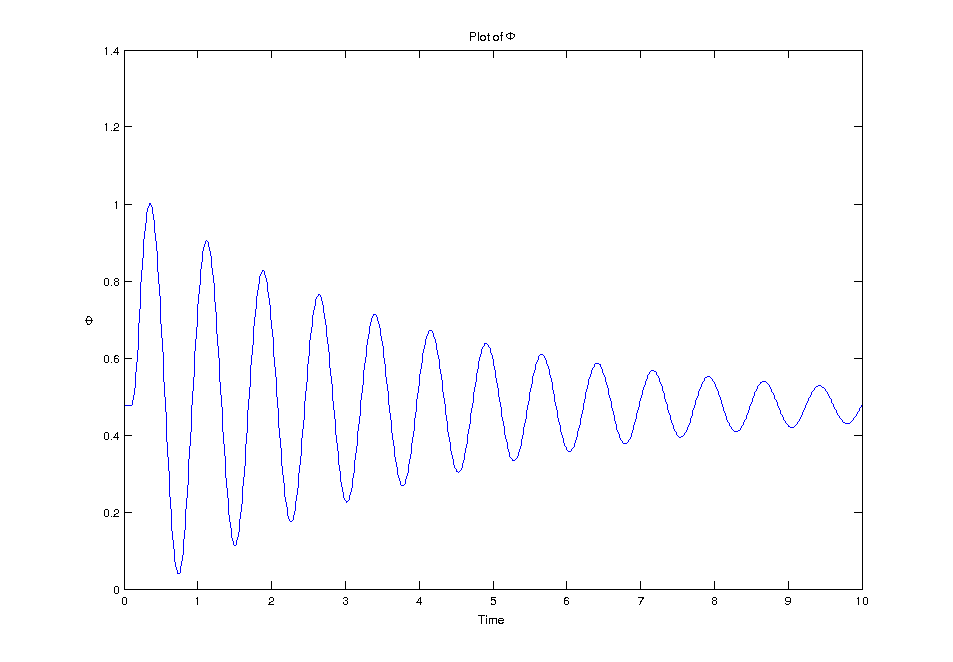
\includegraphics[width=1.2\linewidth]{../Code/miniApps/power_grid/phi_matlab.png}
\label{fig:plot_of_phi_matlab}
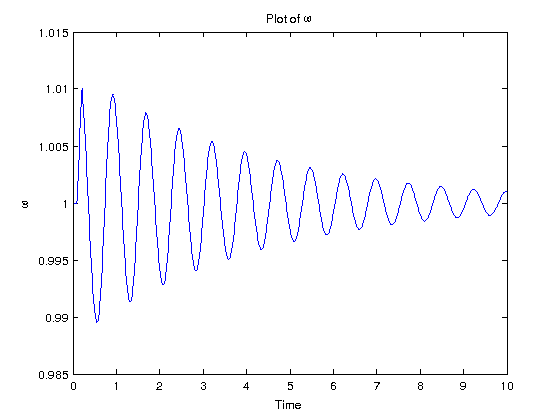
\includegraphics[width=1.2\linewidth]{../Code/miniApps/power_grid/omega_matlab.png}
\label{fig:plot_of_omega_matlab}
\end{figure}
\clearpage
\subsubsection{\texttt{Fortran} port with continuous adjoints}\label{sec_fortran_port_power}
The directory \texttt{Fortran/ContinousAdj} contains the port of the \texttt{MATLAB} version. L-BFGS \cite{Byrd_1996},\cite{Zhu_1997},\cite{Morales_2011} was used to perform the optimization in the \texttt{Fortran} port, a copy of which can be obtained \href{http://users.iems.northwestern.edu/~nocedal/lbfgsb.html}{here}.\\

\noindent The directory \texttt{Fortran/ContinousAdj} contains the files to compile continous adjoint version of the optimal control problem listed in \ref{power_cont_adj_math} and \cite{Rao_2013}. The binaries (\textbf{files}), corresponding to these, on building the directory are \texttt{powergrid} (\textbf{{main.f90}}).\\

\noindent The listing of files and their descriptions follow.\\

\dirtree{%
.1 /. 
.2 Fortran/ContinuousAdj.  
.3 blas.f\DTcomment{L-BFGS support file}. 
.3 constants.f90\DTcomment{Constants and shared variables}. 
.3 gnufor2.f90\DTcomment{\texttt{Fortran} bindings for GNUPlot}. 
.3 iterate.dat\DTcomment{Output from L-BFGS optimization routine}. 
.3 lbfgsb.f\DTcomment{L-BFGS optimization routine}. 
.3 linpack.f\DTcomment{L-BFGS support file}. 
.3 main.f90\DTcomment{Driver for the continuous adjoint port}. 
.3 Makefile\DTcomment{Build commands}. 
.3 print\_active.f\DTcomment{Routines to pretty print matrices and vectors}. 
.3 timer.f\DTcomment{L-BFGS support file}. 
}
\hfill \break
\noindent The plots generated by the \texttt{Fortran} version using continuous adjoints appear on the following page.
\clearpage
\begin{figure}[h]
\centering
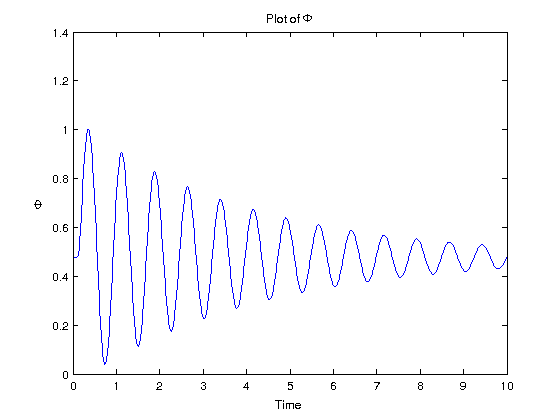
\includegraphics[width=1.2\linewidth]{../Code/miniApps/power_grid/phi_fortran_ca.png}
\label{fig:plot_of_phi_fortran_ca}
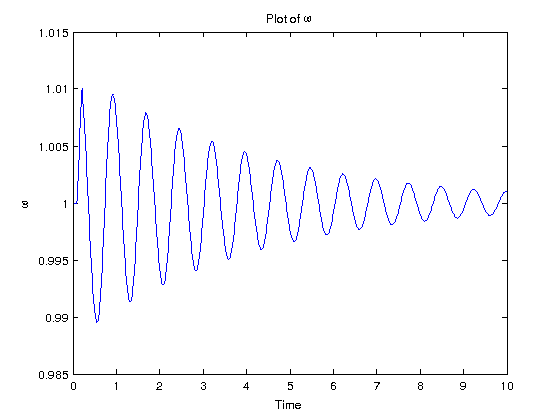
\includegraphics[width=1.2\linewidth]{../Code/miniApps/power_grid/omega_fortran_ca.png}
\label{fig:plot_of_omega_fortran_ca}
\end{figure}
\clearpage
\subsubsection{\texttt{Fortran} port with \texttt{OpenAD/F} in Reverse Split Mode}
For details on reverse split mode refer \cite{Griewank_2008} and \cite{Utke_2014}.\\

\noindent The directory \texttt{Fortran/DiscreteAdj/OpenAD/Split} contains the files to compile the discrete adjoint version of the \texttt{Fortran} port in section \ref{sec_fortran_port_power}. L-BFGS \cite{Byrd_1996},\cite{Zhu_1997},\cite{Morales_2011} was used to perform the optimization in the discrete adjoint version of the Fortran port, a copy of which can be obtained \href{http://users.iems.northwestern.edu/~nocedal/lbfgsb.html}{here}.\\

\noindent The binaries (\textbf{files}), corresponding to these, on building the directory are \texttt{powergrid} (\textbf{{main.f90}}).\\

\noindent The adjoint version of the forward model is used in the file  \texttt{main.f90}. These have been obtained by passing the undifferentiated routines to \texttt{OpenAD/F} in reverse-split mode.\\

\noindent For details on how to call \texttt{OpenAD/F} in reverse-split mode refer \cite{Utke_2014}. The listing of files and their descriptions follow.\\

\dirtree{%
.1 /. 
.2 Fortran/DiscreteAdj/OpenAD/Split.  
.3 blas.f\DTcomment{L-BFGS support file}. 
.3 constants.f90\DTcomment{Constants and shared variables}. 
.3 gnufor2.f90\DTcomment{\texttt{Fortran} bindings for GNUPlot}. 
.3 iterate.dat\DTcomment{Output from L-BFGS optimization routine}. 
.3 lbfgsb.f\DTcomment{L-BFGS optimization routine}. 
.3 linpack.f\DTcomment{L-BFGS support file}. 
.3 main.f90\DTcomment{Driver for the discrete adjoint of port}. 
.3 Makefile\DTcomment{Build commands}. 
.3 Makefile\_continuous\_adjoint\DTcomment{Build commands for CA model}. 
.3 numerics.f90\DTcomment{FW and ADJ model routines from \texttt{main.f90}}. 
.3 print\_active.f\DTcomment{Routines to pretty print matrices and vectors}. 
.3 timer.f\DTcomment{L-BFGS support file}.  
}

\hfill \break
\noindent The plots generated by the \texttt{Fortran} version using discrete adjoints generated by \texttt{OpenAD/F} in reverse-split mode appear on the following page.

\clearpage
\begin{figure}[h]
\centering
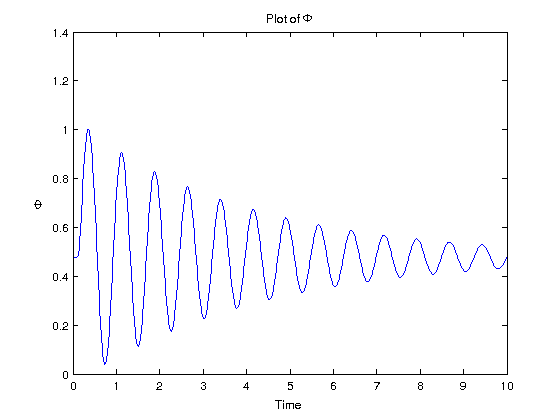
\includegraphics[width=1.2\linewidth]{../Code/miniApps/power_grid/phi_fortran_da_oad_rs.png}
\label{fig:phi_fortran_da_oad_rs}
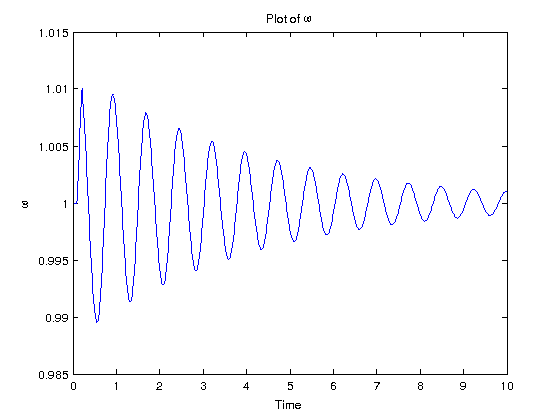
\includegraphics[width=1.2\linewidth]{../Code/miniApps/power_grid/omega_fortran_da_oad_rs.png}
\label{fig:omega_fortran_da_oad_rs}
\end{figure}
\clearpage
\subsubsection{\texttt{Fortran} port with \texttt{OpenAD/F} in Reverse Joint Mode}
For details on reverse joint mode refer \cite{Griewank_2008} and \cite{Utke_2014}.\\

\noindent The directory \texttt{Fortran/DiscreteAdj/OpenAD/Joint} contains the files to compile the discrete adjoint version of the \texttt{Fortran} port in section \ref{sec_fortran_port_power}. L-BFGS \cite{Byrd_1996},\cite{Zhu_1997},\cite{Morales_2011} was used to perform the optimization in the discrete adjoint version of the Fortran port, a copy of which can be obtained \href{http://users.iems.northwestern.edu/~nocedal/lbfgsb.html}{here}.\\

\noindent The binaries (\textbf{files}), corresponding to these, on building the directory are \texttt{powergrid} (\textbf{{main.f90}}).\\

\noindent The adjoint version of the forward model is used in the file  \texttt{main.f90}. These have been obtained by passing the undifferentiated routines to \texttt{OpenAD/F} in reverse-joint mode.\\

\noindent For details on how to call \texttt{OpenAD/F} in reverse-joint mode refer \cite{Utke_2014}. The listing of files and their descriptions follow.\\

\dirtree{%
.1 /. 
.2 Fortran/DiscreteAdj/OpenAD/Joint.  
.3 blas.f\DTcomment{L-BFGS support file}. 
.3 constants.f90\DTcomment{Constants and shared variables}. 
.3 gnufor2.f90\DTcomment{\texttt{Fortran} bindings for GNUPlot}. 
.3 iterate.dat\DTcomment{Output from L-BFGS optimization routine}. 
.3 lbfgsb.f\DTcomment{L-BFGS optimization routine}. 
.3 linpack.f\DTcomment{L-BFGS support file}. 
.3 main.f90\DTcomment{Driver for the discrete adjoint of port}. 
.3 Makefile\DTcomment{Build commands}. 
.3 Makefile\_continuous\_adjoint\DTcomment{Build commands for CA model}. 
.3 numerics.f90\DTcomment{FW and ADJ model routines from \texttt{main.f90}}. 
.3 print\_active.f\DTcomment{Routines to pretty print matrices and vectors}. 
.3 timer.f\DTcomment{L-BFGS support file}.  
}

\hfill \break
\noindent The plots generated by the \texttt{Fortran} version using discrete adjoints generated by \texttt{OpenAD/F} in reverse-joint mode appear on the following page.

\clearpage
\begin{figure}[h]
\centering
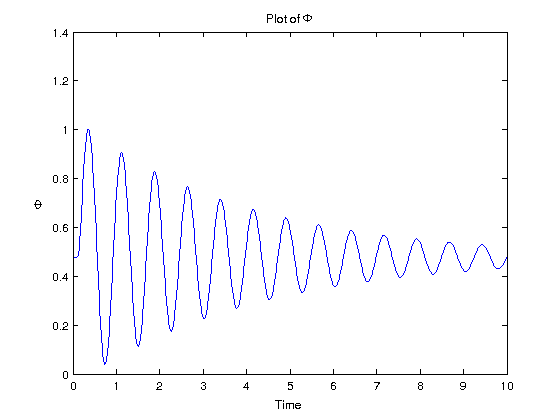
\includegraphics[width=1.2\linewidth]{../Code/miniApps/power_grid/phi_fortran_da_oad_rj.png}
\label{fig:phi_fortran_da_oad_rj}
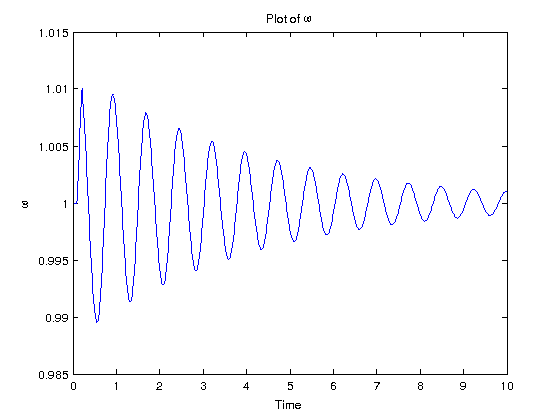
\includegraphics[width=1.2\linewidth]{../Code/miniApps/power_grid/omega_fortran_da_oad_rj.png}
\label{fig:omega_fortran_da_oad_rj}
\end{figure}
\clearpage
\subsubsection{\texttt{Fortran} port with \texttt{OpenAD/F} in Forward Mode}
\noindent The directory \texttt{Fortran/DiscreteAdj/OpenAD/TangLin} contains the files to compile the forward-mode linear version of the \texttt{Fortran} port in section \ref{sec_fortran_port_power}. L-BFGS \cite{Byrd_1996},\cite{Zhu_1997},\cite{Morales_2011} was used to perform the optimization in the discrete adjoint version of the Fortran port, a copy of which can be obtained \href{http://users.iems.northwestern.edu/~nocedal/lbfgsb.html}{here}.\\

\noindent The binaries (\textbf{files}), corresponding to these, on building the directory are \texttt{powergrid} (\textbf{{main.f90}}).\\

\noindent The tangent linear version of the forward model is used in the file  \texttt{main.f90}. These have been obtained by passing the undifferentiated routines to \texttt{OpenAD/F} in forward mode.\\

\noindent For details on how to call \texttt{OpenAD/F} in forward mode refer \cite{Utke_2014}. The listing of files and their descriptions follow.\\

\dirtree{%
.1 /. 
.2 Fortran/DiscreteAdj/OpenAD/Joint.  
.3 blas.f\DTcomment{L-BFGS support file}. 
.3 constants.f90\DTcomment{Constants and shared variables}. 
.3 gnufor2.f90\DTcomment{\texttt{Fortran} bindings for GNUPlot}. 
.3 iterate.dat\DTcomment{Output from L-BFGS optimization routine}. 
.3 lbfgsb.f\DTcomment{L-BFGS optimization routine}. 
.3 linpack.f\DTcomment{L-BFGS support file}. 
.3 main.f90\DTcomment{Driver for the discrete adjoint of port}. 
.3 Makefile\DTcomment{Build commands}. 
.3 Makefile\_continuous\_adjoint\DTcomment{Build commands for CA model}. 
.3 numerics.f90\DTcomment{FW and ADJ model routines from \texttt{main.f90}}. 
.3 print\_active.f\DTcomment{Routines to pretty print matrices and vectors}. 
.3 timer.f\DTcomment{L-BFGS support file}.  
}

\begin{TodoPar}
\noindent Unfortunately, at the time of writing, the tangent-linear version of the forward model does not converge resulting in completely corrupted results. Further the code exhibits a strange behavior, in that it gives yet another completely different result when a single print statement is added after passing it through \texttt{OpenAD/F}. 
\end{TodoPar}

\noindent Quoting verbatim an excerpt of an email that I had written about this behavior (on the following page):
\clearpage
\begin{Verbatim}[xleftmargin=2em]
The numerical routines are all in numerics.f90. 
When I was debugging I noticed that the 
non-linear solve inside Crank Nicolson 
scheme was not converging properly. There is a 
quantity called conv_err which is the convergence 
error. There is an if block which checks whether
the convergence error has fallen below a 
threshold : 1e-8 before moving onto the next time
point in the integrator. 

I was trying to print conv_err (after passing 
through open ad) before the if block. I ensured
that the openad command was disables in the 
makefile. But adding this print changes the 
output when run in comparison to without the
print statement.

The process is as follows:

1) Run Make
2) open the generated numerics.pre....post.f90
3) Add the print statement before the if block 
which check conv_err < 1e-8 inside Crank Nicolson 
scheme
4) Open Makefile
5) Comment out `openad` call
6) Make
7) Run powergrid (result different from without 
adding the print statement in step 3)

The source code is under 
/Code/miniApps/powergrid/DiscreteAdj/OpenAD/TangLin
\end{Verbatim}
\clearpage
\subsection{Modifications performed}
Refer section \ref{diff_airfoil}
\subsection{How to build}
Running make as below, in each of the four subdirectories beginning with ``airfoil'' will build the  binaries \texttt{airfoil}, \texttt{air\_lin} and \texttt{air\_adj}.
\hfill\break
\begin{lstlisting}[language=mybash, numbers=none]
    $ make
\end{lstlisting}
\begin{NotePar}
\noindent  The directories \texttt{air\_foil\_wopenad\_split} and \texttt{air\_foil\_wopenad\_joint} will only build the binaries \texttt{airfoil} and \texttt{air\_adj}.\\

\noindent Likewise the directory \texttt{air\_foil\_wopenad\_tanglin} will only build the binaries \texttt{airfoil} and \texttt{air\_lin}.
\end{NotePar}
\subsection{How to verify}
At the time of writing, there exists no script that can validate the output from any of the binaries. All versions of the binary \texttt{airfoil} should produce exactly the same output.\\

\noindent Validation by eyeballing the output from each version of the binaries \texttt{air\_lin} and  \texttt{air\_adj} has been performed. It is of significance to note that the outputs from \texttt{air\_lin} and  \texttt{air\_adj} should also be within certain fixed tolerance from one another.

\begin{TodoPar}
\noindent It will be valuable to write a \texttt{python} script that will take as input two \texttt{csv} files and find the \texttt{max-norm} of the difference between the corresponding entries. Other norms may also be computed. 
\end{TodoPar}

\noindent In order to test the derivatives, since the code does computations deterministically i.e. there are no convergence related iterations, each version of \texttt{airfoil} can be made to write the computed derivatives to a file and the files themselves can be passed to the \texttt{python} script.\\

\begin{TodoPar}
\noindent Additionally, the binary \texttt{testlinadj} can be used to test linear and adjoint routines in \texttt{air\_foil\_tapenade} directory. And by modifying \texttt{testlinadj.F} suitably - by making use of \texttt{oad\_active} type - in each of the other directories, validation can be performed.
\end{TodoPar}


\subsection{How to extend}
\clearpage 
\section{Power Generation (not Power Grid)}
\subsection{Author and source}
The power generation test-case is derived from the summer project \cite{Rao_2013} at ANL. A copy of the source code, with some minor bug fixes to the original, is included in the \texttt{git} repository as described below. The application is an optimal control problem to `\textit{`maximize the input power to a generator while limiting its mechanical angle oscillation}'' as described in the reference above.
\subsection{Description of the mathematical formulation}\label{power_cont_adj_math}
A general framework for an \textcolor{red}{optimal control} \cite{Sandu_2012} problem is given below:
\[ \theta \,=\, \text{argmin} \;\; \Psi(x, \theta) = \int_{t_0}^{t_F} r\big(x(t), \theta\big)\, dt \,+\, w\big(x(t_F), \theta\big)\]
\[ \text{subject to:} \;\; x' = f(t, x, \theta), \; t_0 \leq t \leq t_F, \; x(t_0) = x_0(\theta) \]
Here, we seek to minimize the cost function $\Psi$ by choosing $\theta$. However, noting that the parameter $\theta$ also decides the value of $x(t_F)$ on which the cost function is dependent. This dependency relation of $x(t_F)$ on $\theta$ comes from the constraint ODE.\\

\noindent Using continuous adjoints, the gradient of the \textcolor{red}{hamiltonian} with respect to the parameters $\theta$ can be written as:

\[\nabla_{\theta} \Psi = w_{\theta}^T\big(x(t_F), \theta\big) + \bigg(\frac{d x_0}{d \theta}\bigg)^T \,.\, \lambda(t_0) +\;\int_{t_0}^{t_F} \bigg(f_{\theta}^T(t, x, \theta) \,.\, \lambda(t) + r_{\theta}^T\big(x,\theta\big)\bigg) dt\]

\noindent The actual problem that is being solved by the power generation example is given below:

\[ p_m \,=\, \text{argmin} \;\; \Psi( p_m, \phi) = - p_m \,+\, c \int_{t_0}^{t_F} \big((\phi - \phi_S)_{+}\big)^4 \, dt\]
subject to: 
\begin{eqnarray*}
\frac{d\phi}{dt} &=& \omega_B (\omega - \omega_S)\\
\frac{d\omega}{dt} &=& \frac{\omega_S}{2H} (p_m - p_{max} sin(\phi) - D(\omega - \omega_S)),\; t_0 \leq t \leq t_F \\
\phi(t_0) &=& sin^{-1}\bigg(\frac{p_m}{p_{max}}\bigg) \\
\omega(t_0) &=& 1 
\end{eqnarray*}
$\omega$: frequency, \, $\phi$: phase angle,\, $p_m$: parameter\\

\noindent The \texttt{MATLAB} code uses continuous adjoints to compute the gradient of the cost function $\Psi$ with respect to the parameter $p_m$.
\clearpage
\subsection{Directory structure and description of files}
The power generation test-case is organized into five subdirectories as shown below:\\
\dirtree{%
.1 /. 
.2 MATLAB\DTcomment{Original MATLAB files with minor bug fixes}. 
.2 Fortran/ContinuousAdj\DTcomment{\texttt{Fortran} port with continuous adjoints}. 
.2 Fortran/DiscreteAdj/OpenAD/TangLin\DTcomment{\texttt{OpenAD/F} in FW Mode}. 
.2 Fortran/DiscreteAdj/OpenAD/Joint\DTcomment{\texttt{OpenAD/F} in RJ Mode}. 
.2 Fortran/DiscreteAdj/OpenAD/Split\DTcomment{\texttt{OpenAD/F} in RS Mode}. 
.2 Fortran/DiscreteAdj/Tapenade\DTcomment{Tapenade in Adjoint Mode}.  
}
\subsubsection{\texttt{MATLAB} version}
The directory \texttt{MATLAB} contains the original files with some minor bug fixes to comply with \cite{Rao_2013} and \cite{Sandu_2012}. The \texttt{MATLAB} version of the code uses the continuous adjoint formulation as mentioned in the earlier references.\\

\noindent The listing of files and their descriptions follow.\\
\dirtree{%
.1 /. 
.2 MATLAB.  
.3 main.m\DTcomment{Driver file for the power generation model}. 
.3 sens\_check.m\DTcomment{Model with continuous adjoint}. 
.3 TSOPF\_Experiments.pdf\DTcomment{Same as \cite{Rao_2013}}. 
}
\hfill\break
\noindent The \texttt{MATLAB} version can be executed like below.\\

\begin{lstlisting}[language=mymatlab, numbers=none]
>> main
\end{lstlisting}
\hfill \break
\noindent The plots generated by the \texttt{MATLAB} version appear on the following page.
\clearpage
\begin{figure}[h]
\centering
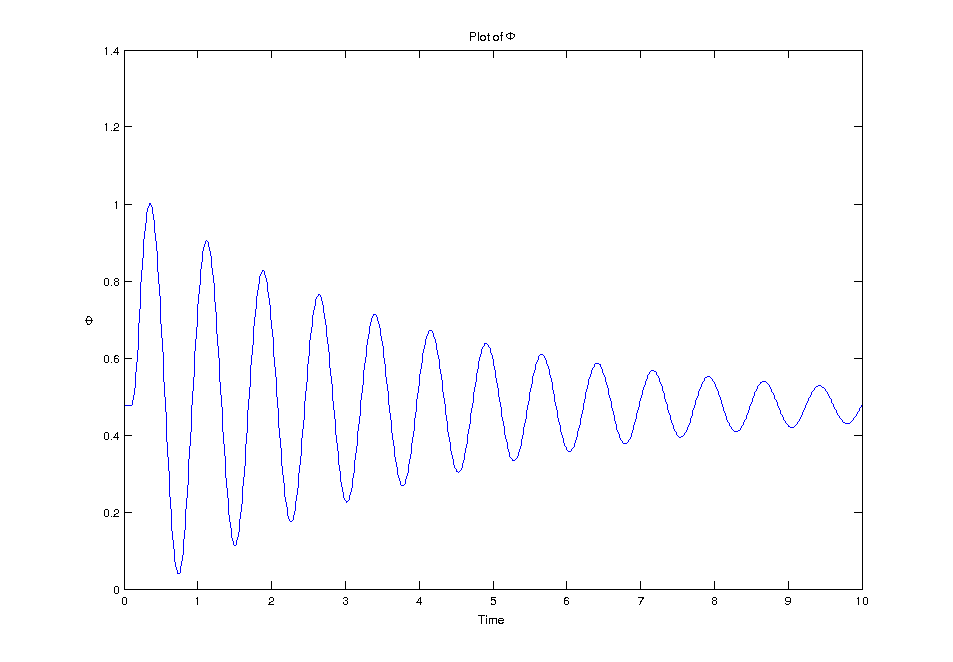
\includegraphics[width=1.2\linewidth]{../Code/miniApps/power_grid/phi_matlab.png}
\label{fig:plot_of_phi_matlab}
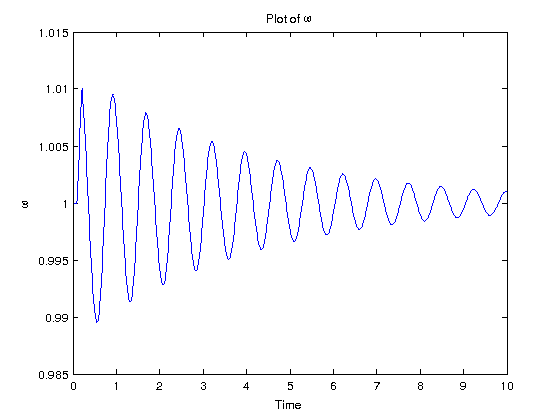
\includegraphics[width=1.2\linewidth]{../Code/miniApps/power_grid/omega_matlab.png}
\label{fig:plot_of_omega_matlab}
\end{figure}
\clearpage
\subsubsection{\texttt{Fortran} port with continuous adjoints}\label{sec_fortran_port_power}
The directory \texttt{Fortran/ContinousAdj} contains the port of the \texttt{MATLAB} version. L-BFGS \cite{Byrd_1996},\cite{Zhu_1997},\cite{Morales_2011} was used to perform the optimization in the \texttt{Fortran} port, a copy of which can be obtained \href{http://users.iems.northwestern.edu/~nocedal/lbfgsb.html}{here}.\\

\noindent The directory \texttt{Fortran/ContinousAdj} contains the files to compile continous adjoint version of the optimal control problem listed in \ref{power_cont_adj_math} and \cite{Rao_2013}. The binaries (\textbf{files}), corresponding to these, on building the directory are \texttt{powergrid} (\textbf{{main.f90}}).\\

\noindent The listing of files and their descriptions follow.\\

\dirtree{%
.1 /. 
.2 Fortran/ContinuousAdj.  
.3 blas.f\DTcomment{L-BFGS support file}. 
.3 constants.f90\DTcomment{Constants and shared variables}. 
.3 gnufor2.f90\DTcomment{\texttt{Fortran} bindings for GNUPlot}. 
.3 iterate.dat\DTcomment{Output from L-BFGS optimization routine}. 
.3 lbfgsb.f\DTcomment{L-BFGS optimization routine}. 
.3 linpack.f\DTcomment{L-BFGS support file}. 
.3 main.f90\DTcomment{Driver for the continuous adjoint port}. 
.3 Makefile\DTcomment{Build commands}. 
.3 print\_active.f\DTcomment{Routines to pretty print matrices and vectors}. 
.3 timer.f\DTcomment{L-BFGS support file}. 
}
\hfill \break
\noindent The plots generated by the \texttt{Fortran} version using continuous adjoints appear on the following page.
\clearpage
\begin{figure}[h]
\centering
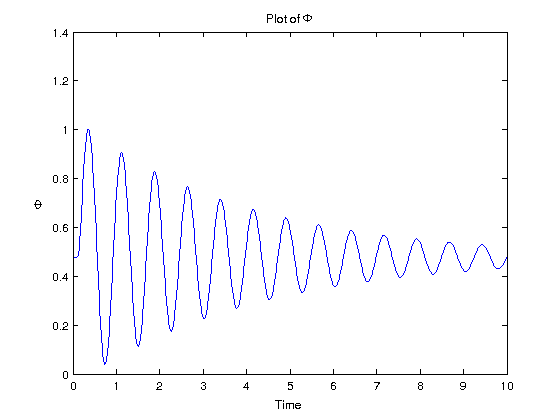
\includegraphics[width=1.2\linewidth]{../Code/miniApps/power_grid/phi_fortran_ca.png}
\label{fig:plot_of_phi_fortran_ca}
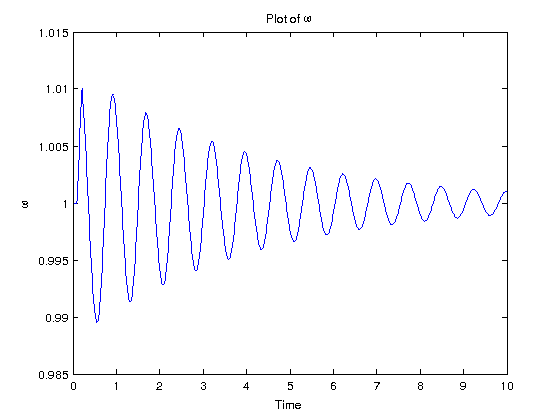
\includegraphics[width=1.2\linewidth]{../Code/miniApps/power_grid/omega_fortran_ca.png}
\label{fig:plot_of_omega_fortran_ca}
\end{figure}
\clearpage
\subsubsection{\texttt{Fortran} port with \texttt{OpenAD/F} in Reverse Split Mode}
For details on reverse split mode refer \cite{Griewank_2008} and \cite{Utke_2014}.\\

\noindent The directory \texttt{Fortran/DiscreteAdj/OpenAD/Split} contains the files to compile the discrete adjoint version of the \texttt{Fortran} port in section \ref{sec_fortran_port_power}. L-BFGS \cite{Byrd_1996},\cite{Zhu_1997},\cite{Morales_2011} was used to perform the optimization in the discrete adjoint version of the Fortran port, a copy of which can be obtained \href{http://users.iems.northwestern.edu/~nocedal/lbfgsb.html}{here}.\\

\noindent The binaries (\textbf{files}), corresponding to these, on building the directory are \texttt{powergrid} (\textbf{{main.f90}}).\\

\noindent The adjoint version of the forward model is used in the file  \texttt{main.f90}. These have been obtained by passing the undifferentiated routines to \texttt{OpenAD/F} in reverse-split mode.\\

\noindent For details on how to call \texttt{OpenAD/F} in reverse-split mode refer \cite{Utke_2014}. The listing of files and their descriptions follow.\\

\dirtree{%
.1 /. 
.2 Fortran/DiscreteAdj/OpenAD/Split.  
.3 blas.f\DTcomment{L-BFGS support file}. 
.3 constants.f90\DTcomment{Constants and shared variables}. 
.3 gnufor2.f90\DTcomment{\texttt{Fortran} bindings for GNUPlot}. 
.3 iterate.dat\DTcomment{Output from L-BFGS optimization routine}. 
.3 lbfgsb.f\DTcomment{L-BFGS optimization routine}. 
.3 linpack.f\DTcomment{L-BFGS support file}. 
.3 main.f90\DTcomment{Driver for the discrete adjoint of port}. 
.3 Makefile\DTcomment{Build commands}. 
.3 Makefile\_continuous\_adjoint\DTcomment{Build commands for CA model}. 
.3 numerics.f90\DTcomment{FW and ADJ model routines from \texttt{main.f90}}. 
.3 print\_active.f\DTcomment{Routines to pretty print matrices and vectors}. 
.3 timer.f\DTcomment{L-BFGS support file}.  
}

\hfill \break
\noindent The plots generated by the \texttt{Fortran} version using discrete adjoints generated by \texttt{OpenAD/F} in reverse-split mode appear on the following page.

\clearpage
\begin{figure}[h]
\centering
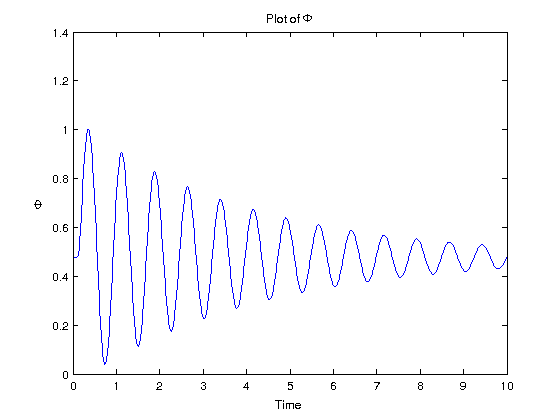
\includegraphics[width=1.2\linewidth]{../Code/miniApps/power_grid/phi_fortran_da_oad_rs.png}
\label{fig:phi_fortran_da_oad_rs}
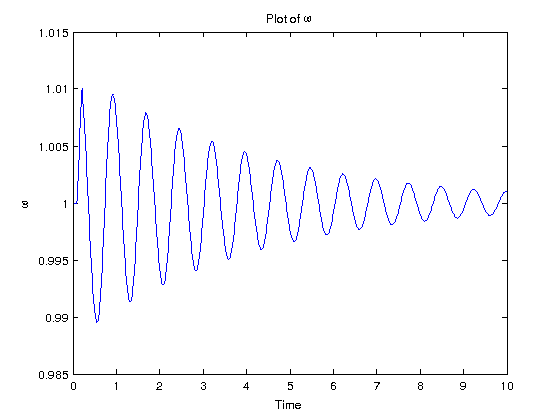
\includegraphics[width=1.2\linewidth]{../Code/miniApps/power_grid/omega_fortran_da_oad_rs.png}
\label{fig:omega_fortran_da_oad_rs}
\end{figure}
\clearpage
\subsubsection{\texttt{Fortran} port with \texttt{OpenAD/F} in Reverse Joint Mode}
For details on reverse joint mode refer \cite{Griewank_2008} and \cite{Utke_2014}.\\

\noindent The directory \texttt{Fortran/DiscreteAdj/OpenAD/Joint} contains the files to compile the discrete adjoint version of the \texttt{Fortran} port in section \ref{sec_fortran_port_power}. L-BFGS \cite{Byrd_1996},\cite{Zhu_1997},\cite{Morales_2011} was used to perform the optimization in the discrete adjoint version of the Fortran port, a copy of which can be obtained \href{http://users.iems.northwestern.edu/~nocedal/lbfgsb.html}{here}.\\

\noindent The binaries (\textbf{files}), corresponding to these, on building the directory are \texttt{powergrid} (\textbf{{main.f90}}).\\

\noindent The adjoint version of the forward model is used in the file  \texttt{main.f90}. These have been obtained by passing the undifferentiated routines to \texttt{OpenAD/F} in reverse-joint mode.\\

\noindent For details on how to call \texttt{OpenAD/F} in reverse-joint mode refer \cite{Utke_2014}. The listing of files and their descriptions follow.\\

\dirtree{%
.1 /. 
.2 Fortran/DiscreteAdj/OpenAD/Joint.  
.3 blas.f\DTcomment{L-BFGS support file}. 
.3 constants.f90\DTcomment{Constants and shared variables}. 
.3 gnufor2.f90\DTcomment{\texttt{Fortran} bindings for GNUPlot}. 
.3 iterate.dat\DTcomment{Output from L-BFGS optimization routine}. 
.3 lbfgsb.f\DTcomment{L-BFGS optimization routine}. 
.3 linpack.f\DTcomment{L-BFGS support file}. 
.3 main.f90\DTcomment{Driver for the discrete adjoint of port}. 
.3 Makefile\DTcomment{Build commands}. 
.3 Makefile\_continuous\_adjoint\DTcomment{Build commands for CA model}. 
.3 numerics.f90\DTcomment{FW and ADJ model routines from \texttt{main.f90}}. 
.3 print\_active.f\DTcomment{Routines to pretty print matrices and vectors}. 
.3 timer.f\DTcomment{L-BFGS support file}.  
}

\hfill \break
\noindent The plots generated by the \texttt{Fortran} version using discrete adjoints generated by \texttt{OpenAD/F} in reverse-joint mode appear on the following page.

\clearpage
\begin{figure}[h]
\centering
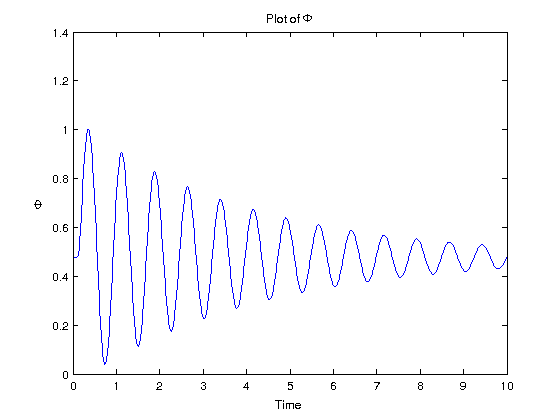
\includegraphics[width=1.2\linewidth]{../Code/miniApps/power_grid/phi_fortran_da_oad_rj.png}
\label{fig:phi_fortran_da_oad_rj}
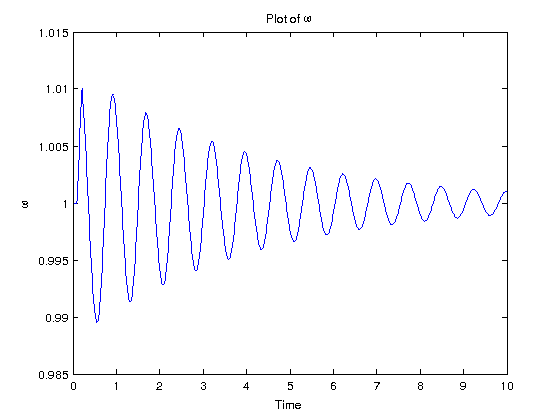
\includegraphics[width=1.2\linewidth]{../Code/miniApps/power_grid/omega_fortran_da_oad_rj.png}
\label{fig:omega_fortran_da_oad_rj}
\end{figure}
\clearpage
\subsubsection{\texttt{Fortran} port with \texttt{OpenAD/F} in Forward Mode}
\noindent The directory \texttt{Fortran/DiscreteAdj/OpenAD/TangLin} contains the files to compile the forward-mode linear version of the \texttt{Fortran} port in section \ref{sec_fortran_port_power}. L-BFGS \cite{Byrd_1996},\cite{Zhu_1997},\cite{Morales_2011} was used to perform the optimization in the discrete adjoint version of the Fortran port, a copy of which can be obtained \href{http://users.iems.northwestern.edu/~nocedal/lbfgsb.html}{here}.\\

\noindent The binaries (\textbf{files}), corresponding to these, on building the directory are \texttt{powergrid} (\textbf{{main.f90}}).\\

\noindent The tangent linear version of the forward model is used in the file  \texttt{main.f90}. These have been obtained by passing the undifferentiated routines to \texttt{OpenAD/F} in forward mode.\\

\noindent For details on how to call \texttt{OpenAD/F} in forward mode refer \cite{Utke_2014}. The listing of files and their descriptions follow.\\

\dirtree{%
.1 /. 
.2 Fortran/DiscreteAdj/OpenAD/Joint.  
.3 blas.f\DTcomment{L-BFGS support file}. 
.3 constants.f90\DTcomment{Constants and shared variables}. 
.3 gnufor2.f90\DTcomment{\texttt{Fortran} bindings for GNUPlot}. 
.3 iterate.dat\DTcomment{Output from L-BFGS optimization routine}. 
.3 lbfgsb.f\DTcomment{L-BFGS optimization routine}. 
.3 linpack.f\DTcomment{L-BFGS support file}. 
.3 main.f90\DTcomment{Driver for the discrete adjoint of port}. 
.3 Makefile\DTcomment{Build commands}. 
.3 Makefile\_continuous\_adjoint\DTcomment{Build commands for CA model}. 
.3 numerics.f90\DTcomment{FW and ADJ model routines from \texttt{main.f90}}. 
.3 print\_active.f\DTcomment{Routines to pretty print matrices and vectors}. 
.3 timer.f\DTcomment{L-BFGS support file}.  
}

\begin{TodoPar}
\noindent Unfortunately, at the time of writing, the tangent-linear version of the forward model does not converge resulting in completely corrupted results. Further the code exhibits a strange behavior, in that it gives yet another completely different result when a single print statement is added after passing it through \texttt{OpenAD/F}. 
\end{TodoPar}

\noindent Quoting verbatim an excerpt of an email that I had written about this behavior (on the following page):
\clearpage
\begin{Verbatim}[xleftmargin=2em]
The numerical routines are all in numerics.f90. 
When I was debugging I noticed that the 
non-linear solve inside Crank Nicolson 
scheme was not converging properly. There is a 
quantity called conv_err which is the convergence 
error. There is an if block which checks whether
the convergence error has fallen below a 
threshold : 1e-8 before moving onto the next time
point in the integrator. 

I was trying to print conv_err (after passing 
through open ad) before the if block. I ensured
that the openad command was disables in the 
makefile. But adding this print changes the 
output when run in comparison to without the
print statement.

The process is as follows:

1) Run Make
2) open the generated numerics.pre....post.f90
3) Add the print statement before the if block 
which check conv_err < 1e-8 inside Crank Nicolson 
scheme
4) Open Makefile
5) Comment out `openad` call
6) Make
7) Run powergrid (result different from without 
adding the print statement in step 3)

The source code is under 
/Code/miniApps/powergrid/DiscreteAdj/OpenAD/TangLin
\end{Verbatim}
\clearpage
\subsection{Modifications performed}
Refer section \ref{diff_airfoil}
\subsection{How to build}
Running make as below, in each of the four subdirectories beginning with ``airfoil'' will build the  binaries \texttt{airfoil}, \texttt{air\_lin} and \texttt{air\_adj}.
\hfill\break
\begin{lstlisting}[language=mybash, numbers=none]
    $ make
\end{lstlisting}
\begin{NotePar}
\noindent  The directories \texttt{air\_foil\_wopenad\_split} and \texttt{air\_foil\_wopenad\_joint} will only build the binaries \texttt{airfoil} and \texttt{air\_adj}.\\

\noindent Likewise the directory \texttt{air\_foil\_wopenad\_tanglin} will only build the binaries \texttt{airfoil} and \texttt{air\_lin}.
\end{NotePar}
\subsection{How to verify}
At the time of writing, there exists no script that can validate the output from any of the binaries. All versions of the binary \texttt{airfoil} should produce exactly the same output.\\

\noindent Validation by eyeballing the output from each version of the binaries \texttt{air\_lin} and  \texttt{air\_adj} has been performed. It is of significance to note that the outputs from \texttt{air\_lin} and  \texttt{air\_adj} should also be within certain fixed tolerance from one another.

\begin{TodoPar}
\noindent It will be valuable to write a \texttt{python} script that will take as input two \texttt{csv} files and find the \texttt{max-norm} of the difference between the corresponding entries. Other norms may also be computed. 
\end{TodoPar}

\noindent In order to test the derivatives, since the code does computations deterministically i.e. there are no convergence related iterations, each version of \texttt{airfoil} can be made to write the computed derivatives to a file and the files themselves can be passed to the \texttt{python} script.\\

\begin{TodoPar}
\noindent Additionally, the binary \texttt{testlinadj} can be used to test linear and adjoint routines in \texttt{air\_foil\_tapenade} directory. And by modifying \texttt{testlinadj.F} suitably - by making use of \texttt{oad\_active} type - in each of the other directories, validation can be performed.
\end{TodoPar}


\subsection{How to extend}
 \clearpage

\newpage
\bibliographystyle{acm}
\bibliography{report}  

\newpage
\vfill
\begin{flushright}
\scriptsize
\framebox{\parbox{2.4in}{The submitted manuscript has been created by
UChicago Argonne, LLC, Operator of Argonne National Laboratory
(``Argonne").  Argonne, a U.S. Department of Energy Office
of Science laboratory, is operated under Contract No.
DE-AC02-06CH11357.  The U.S. Government retains for itself, and
others acting on its behalf, a paid-up, nonexclusive, irrevocable
worldwide license in said article to reproduce, prepare derivative works,
distribute copies to the public, and perform publicly and display
publicly, by or on behalf of the Government.}}
\normalsize
\end{flushright}

% that's all folks
\end{document}


